\chapter{Architektur des Protokolls}
\label{chap:entwurf_und_architektur}

In diesem Kapitel wird die Architektur des Protokolls entwickelt. Dazu wird zunächst eine geeignete Peer-to-Peer-Technologie ausgewählt. Anschließend wird die darauf aufbauende Peer-Discovery und das Routing betrachtet. Danach wird das Verbindungsmanagement, welches den Verbindungsaufbau, die Nachrichtenübertragung und den Verbindungsabbau beinhaltet, definiert. Darauf folgt ein Vorschlag einer Definition für eine Ende-zu-Ende-Verschlüsselung, welche die Vertraulichkeit der Nachrichten gewährleistet. Abschließend werden verschiedene Möglichkeiten zur Integration der Blockchain in das Protokoll besprochen und eine davon ausgewählt.


\section{Auswahl der Peer-to-Peer-Technologie}
\label{sec:grundlagen_des_protokolls}

Das Tox-Protokoll, das auch auf Peer-to-Peer-Technologie aufbaut (siehe \ref{subsubsection:tox} \textit{\nameref{subsubsection:tox}}), verwendet zur Auffindung der Teilnehmer verteilte Hashtabellen \Parencite{tox_spec}. Da dies eine effiziente Möglichkeit ist, um Teilnehmer zu finden, wird diese Technologie auch für das Protokoll dieser Arbeit verwendet. Verteilte Hashtabellen haben allerdings den Nachteil, das der Verbindungsaufbau im modernen Internet durch NATs erschwert wird. Deshalb wird für das entwickelte Protokoll ein mehrstufiger Ansatz verwendet. In den folgenden Abschnitten wird der Ansatz erläutert und die verwendeten Technologien beschrieben.

Für den effizienten Aufbau einer Direktverbindung zwischen zwei Teilnehmern kamen Chord und Kademlia in die engere Auswahl, welche beide lange Gegenstand intensiver Forschung waren, sowohl in der Industrie als auch in der akademischen Welt \parencite[S. 808]{MedranoChavez_ChordKademliaHighChurnScenarios}. 
Das Chord-Protokoll und das Kademlia-Protokoll sind zwei grundlegend verschiedene Ansätze zur Organisation von Peer-to-Peer-Netzwerken. Beide Protokolle sind strukturiert und bieten eine effiziente Ressourcenlokalisierung, aber sie unterscheiden sich in ihrer Routing-Struktur und der Art und Weise, wie sie die Knoteninformationen verwalten.

\subsubsection{Chord}
Chord basiert auf einer Ringstruktur (siehe Abbildung \ref{chord_ring}), bei der die Knoten in einem Ring angeordnet sind und jeder Knoten für einen bestimmten Schlüsselbereich verantwortlich ist. Die Verbindungen zwischen den Knoten sind durch ihren Platz im Ring definiert, wobei jeder Knoten eine Verbindung zu seinem nächsten Nachbarn im Uhrzeigersinn hat. Ein Knoten besitzt zwei Informationsmengen: eine \textit{Successor-Liste} und eine \textit{Finger-Tabelle}. Die Successor-Liste enthält die Knoten, die direkt nach dem Knoten im Uhrzeigersinn im Ring kommen. Die Anzahl der dort enthaltenen Knoten hängt davon ab, wie viele Knoten im Netzwerk insgesamt vorhanden sind. Die Finger-Tabelle enthält die Knoten, die für die Schlüsselbereiche verantwortlich sind, die durch eine Berechnung auf der ID des Knotens basieren \Parencite[S. 810-811]{MedranoChavez_ChordKademliaHighChurnScenarios}.

Wenn das Chord-Netzwerk eine Suchanfrage erhält, gibt es zwei Strategien, um die Anfrage zu bearbeiten. In der ersten Strategie wird die Anfrage sequentiell von Knoten zu Knoten weitergeleitet, bis der Knoten gefunden wird, der für den Schlüsselbereich verantwortlich ist, in dem sich der gesuchte Schlüssel befindet. Für diese Suchstrategie ergibt sich daher eine Komplexität von $\mathcal{O}(n)$, wobei $n$ die Anzahl der Knoten im Netzwerk ist. $\mathcal{O}(n)$ beschreibt eine lineare Komplexität. Das bedeutet, dass die Anzahl der Weiterleitungen von der Anzahl der Knoten im Netzwerk abhängt \parencite[S. 810-811]{MedranoChavez_ChordKademliaHighChurnScenarios}.

Die zweite Strategie verwendet die Finger-Tabelle, um die Anzahl der Knoten zu reduzieren, die die Anfrage weiterleiten. Diese Strategie hat eine Komplexität von $\mathcal{O}(\log n)$, wobei $n$ die Anzahl der Knoten im Netzwerk ist. Hier beschreibt $\mathcal{O}(\log n)$ eine logarithmische Komplexität. Das bedeutet, dass die Anzahl der Weiterleitungen von der Anzahl der Knoten im Netzwerk abhängt, aber nicht linear, sondern logarithmisch. Dies ist eine effizientere Strategie als die sequentielle Weiterleitung \parencite[S. 810-811]{MedranoChavez_ChordKademliaHighChurnScenarios}.

\begin{center}
    \captionsetup{type=figure}
    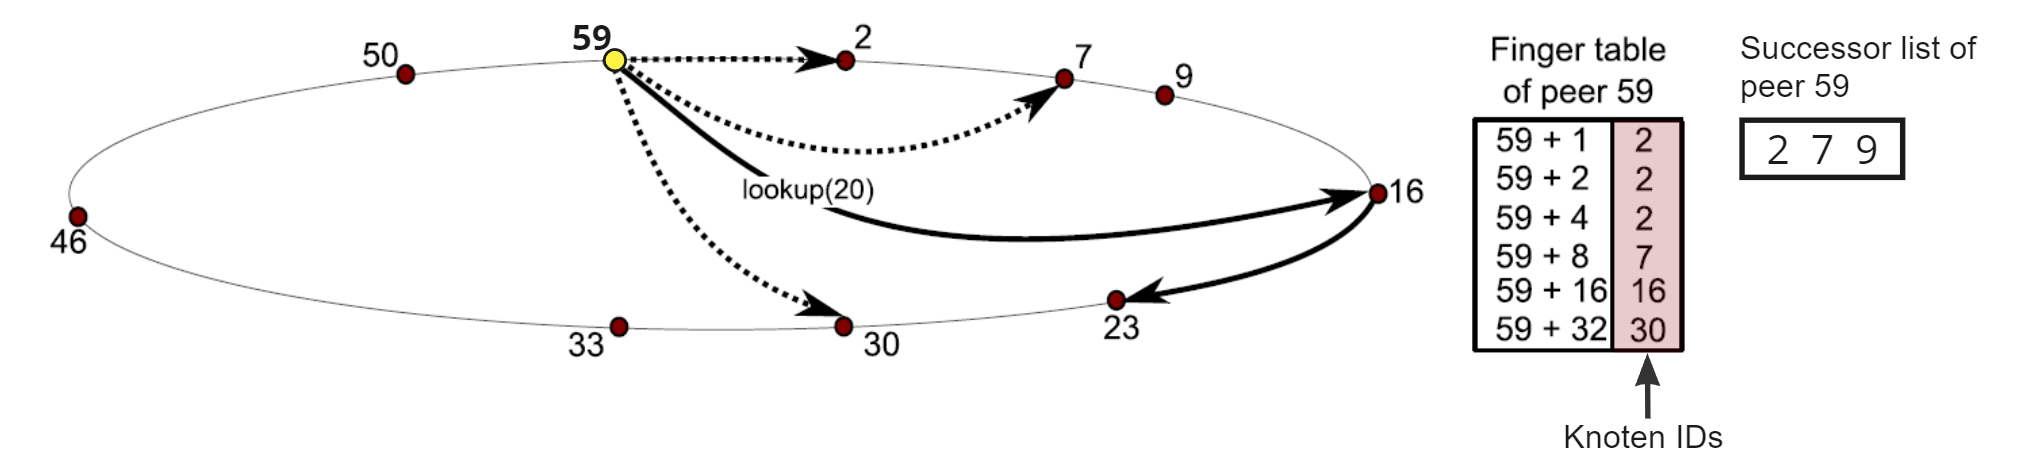
\includegraphics[width=1\linewidth]{images/chord_ring_altered.png}
    \captionof{figure}{Visualisierung einer Suche in der Ringstruktur von Chord (in Anlehnung an \cite[S. 811]{MedranoChavez_ChordKademliaHighChurnScenarios})}
    \label{chord_ring}
\end{center}

\noindent In Abbildung \ref{chord_ring} ist zu erkennen, dass Knoten $59$ eine Suchanfrage für den Knoten mit der ID $20$ beginnt. Unter Verwendung der Finger-Tabelle von Knoten $59$ wird die Anfrage an den Knoten gesendet, der am nächsten an Knoten $20$ liegt. In diesem Fall ist dies Knoten $16$. Knoten $16$ wiederum leitet die Anfrage an den Knoten weiter, der ebenfalls am nächsten an Knoten $20$ liegt, was Knoten $23$ ist. Knoten $23$ ist für den Schlüsselbereich verantwortlich, in dem sich der gesuchte Schlüssel befindet, und sendet daher die Antwort an Knoten $59$ zurück. Durch die Verwendung dieser Strategie wurde Knoten $20$ in nur zwei Schritten gefunden, anstatt in fünft Schritten, wenn die Anfrage sequentiell weitergeleitet worden wäre.    

\subsubsection{Kademlia}
Im Gegensatz zu Chord verwendet Kademlia eine k-Bucket-Struktur, die in Abbildung \ref{kademlia_tree} zu sehen ist, um eine effiziente Verwaltung von Knoteninformationen zu ermöglichen. Die k-Buckets enthalten eine Liste von Knoten für verschiedene Schlüsselbereiche basierend auf ihrer Nähe, die durch XOR-Distanzen der IDs berechnet wird. Die Verbindungen zwischen den Knoten sind asymmetrisch (siehe \ref{subsec:kademlia_vs_chord_vs_pastry} \textit{\nameref{subsec:kademlia_vs_chord_vs_pastry}}), und jeder Knoten speichert Informationen über andere Knoten in seinen k-Buckets. Bei der Suche nach einem bestimmten Schlüssel erfolgt das Routing durch die XOR-Entfernung, wodurch die nächsten Knoten für diesen Schlüssel gefunden werden.
% asymmetrisch -> Knoten A kann Knoten B kennen, aber Knoten B kennt Knoten A nicht

\begin{center}
    \captionsetup{type=figure}
    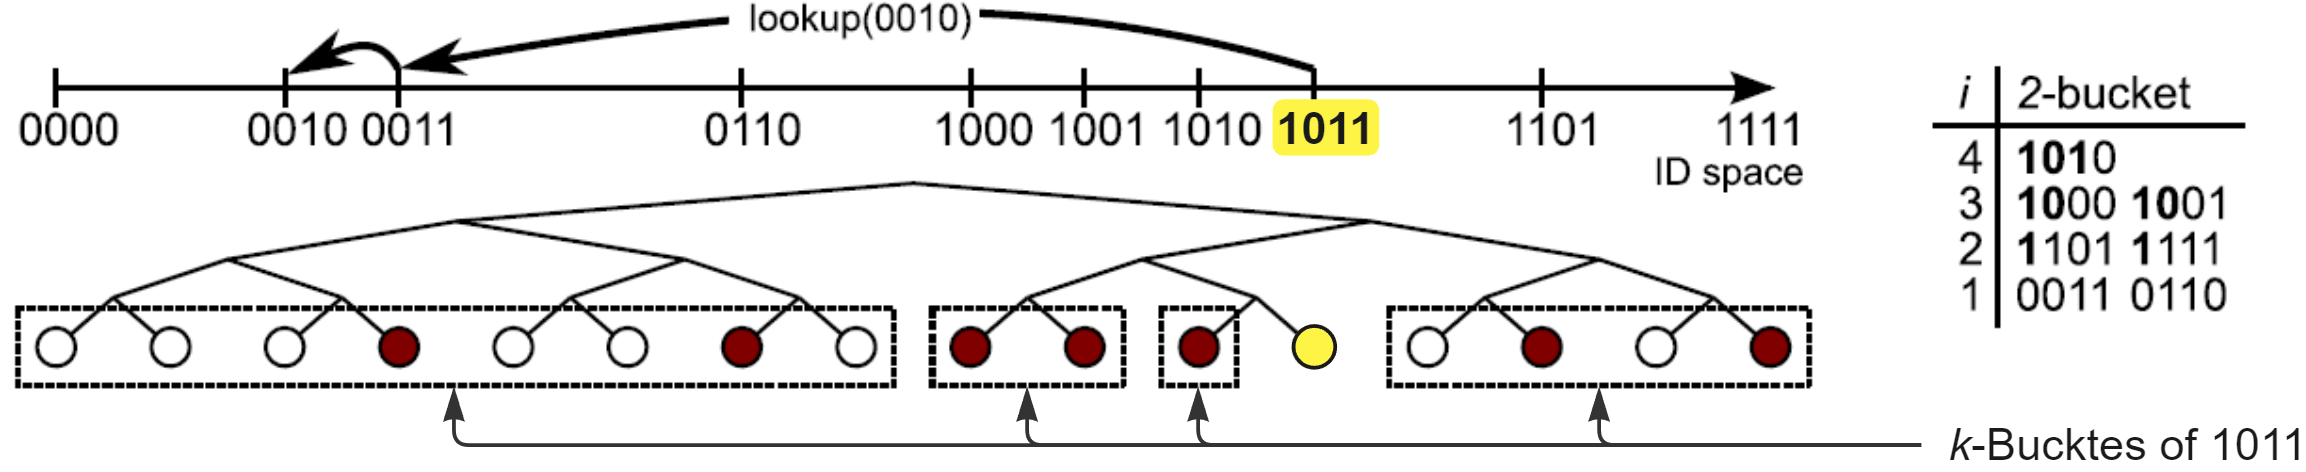
\includegraphics[width=1\linewidth]{images/kademlia_tree_altered.png}
    \captionof{figure}{Visualisierung der Baumstruktur von Kademlia, in Anlehnung an \cite[S. 812]{MedranoChavez_ChordKademliaHighChurnScenarios}}
    \label{kademlia_tree}
\end{center}

\noindent In Abbildung \ref{kademlia_tree} ist zu sehen, wie der Knoten $1011$ ein Suche nach Knoten $0010$ startet. Der Knoten $1011$ sucht in seinen vier Buckets nach dem nächsten Knoten, der am Schlüssel $0010$ liegt. Im ersten Bucket sind Knoten mit dem Präfix $0xxx$ enthalten. In Bucket zwei sind Knoten mit dem Präfix $11xx$, in Bucket drei Knoten mit dem Präfix $100x$ und in Bucket vier Knoten mit dem Präfix $101x$. Da der Schlüssel $0010$ mit dem Präfix $00$ beginnt, wird der nächste Knoten für diesen Schlüssel im ersten Bucket gesucht. Knoten $0011$ wird als nächster Knoten für den Schlüssel $0010$ gefunden. Knoten $1011$ sendet die Anfrage also an Knoten $0011$, der wiederum den nächsten Knoten für den Schlüssel $0010$ sucht. Da dieser Knoten den Schlüssel $0010$ in einem seiner Buckets besitzt, sendet er die Antwort auf die Suchanfrage an Knoten $1011$ zurück. Es werden zwei Weiterleitungen durchgeführt, um den Zielknoten zu finden, woraus sich eine Komplexität von $\mathcal{O}(\log n)$ ergibt, wobei $n$ die Anzahl der Knoten im Netzwerk ist. Dies stellt, wie bereits erwähnt, eine logarithmische Komplexität dar, was bedeutet, dass die Anzahl der Weiterleitungen von der Anzahl der Knoten im Netzwerk abhängt, aber nicht linear, sondern logarithmisch. Dies wiederum bedeutet, dass die Anzahl der Weiterleitungen bei einer großen Anzahl von Knoten im Netzwerk nicht stark ansteigt \Parencite[S. 812]{MedranoChavez_ChordKademliaHighChurnScenarios}.


Funktionen, wie diese Suche, werden durch die vier Nachrichten \textit{FIND\_NODE}, \\\textit{FIND\_VALUE}, \textit{PING} und \textit{STORE} des Kademlia-Protokolls ermöglicht. Sie haben die folgende Verwendung \Parencite[S. 3]{Maymounkov_Kademlia}:

\begin{itemize}
    \item \textit{FIND\_NODE}: Diese Nachricht wird verwendet, um den nächsten Knoten für einen bestimmten Schlüssel zu finden. Sie wird von einem Knoten an einen anderen Knoten gesendet, der den Schlüssel in seinem k-Bucket hat. Der Knoten, der die Nachricht erhält, antwortet mit einer Liste von Knoten, die den Schlüssel in ihrem k-Bucket haben \Parencite[S. 3]{Maymounkov_Kademlia}. 
    \item \textit{FIND\_VALUE}: Diese Nachricht wird verwendet, um den Wert für einen bestimmten Schlüssel zu finden. Sie wird von einem Knoten an einen anderen Knoten gesendet, der den Schlüssel in seinem k-Bucket hat. Der Knoten, der die Nachricht erhält, antwortet mit dem Wert, der dem Schlüssel zugeordnet ist, oder mit einer Liste von Knoten, die den Schlüssel in ihrem k-Bucket haben \Parencite[S. 3]{Maymounkov_Kademlia}.
    \item \textit{PING}: Diese Nachricht wird verwendet, um die Erreichbarkeit eines Knotens zu überprüfen. Sie wird von einem Knoten an einen anderen Knoten gesendet, um zu überprüfen, ob der Knoten noch erreichbar ist \Parencite[S. 2-3]{Maymounkov_Kademlia}.
    \item \textit{STORE}: Diese Nachricht wird verwendet, um einen Schlüssel-Wert-Paar in einem k-Bucket zu speichern. Sie wird von einem Knoten an einen anderen Knoten gesendet, um den Schlüssel-Wert-Paar in seinem k-Bucket zu speichern. Der Knoten, der die Nachricht erhält, speichert den Schlüssel-Wert-Paar in seinem k-Bucket \Parencite[S. 3]{Maymounkov_Kademlia}.
\end{itemize}

\noindent Da bei einem Instant-Messaging-Protokoll häufig Teilnehmer das Netzwerk verlassen und neue Teilnehmer dem Netzwerk beitreten, ist es wichtig, dass das Protokoll mit hoher Fluktuation umgehen kann. Diese Fluktuation von Nodes wird als Churn bezeichnet. In einer Studie von Medrano-Chávez et al. \parencite{MedranoChavez_ChordKademliaHighChurnScenarios}, welche im hybriden Journal \textit{Peer-to-Peer Networking and Applications} veröffentlicht wurde, wurde die Leistung von Chord und Kademlia in Bezug auf Netzwerkfluktuation untersucht. 

\begin{center}
    \captionsetup{type=figure}
    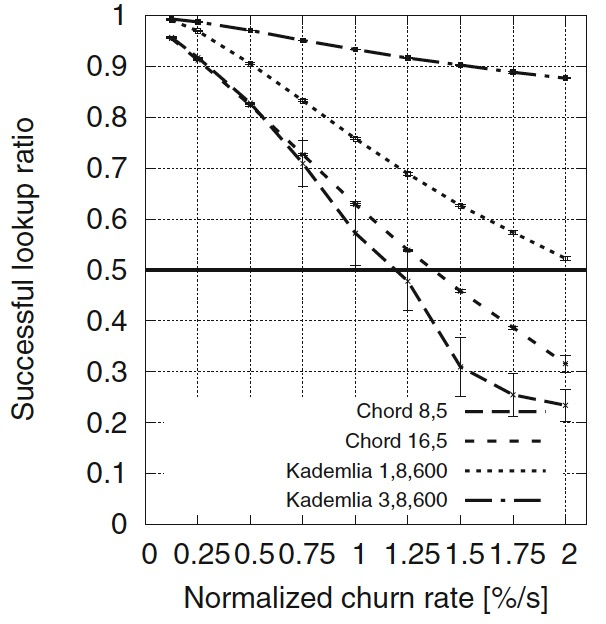
\includegraphics[width=0.5\linewidth]{images/kademlia_chord_churn.jpg}
    \captionof{figure}{Vergleich der Leistung von Chord und Kademlia bei hoher Fluktuation \parencite[S. 818]{MedranoChavez_ChordKademliaHighChurnScenarios}}
    \label{chord_kademlia_churn}
\end{center}

\noindent In Abbildung \ref{chord_kademlia_churn} ist ein Graph zu sehen, auf dem vier Linien zu sehen sind. Auf der x-Achse ist die ist die Churn-Rate in Fluktuationen pro Sekunde aufgetragen. Auf der y-Achse ist das Verhältnis der erfolgreichen Suchanfragen zur Anzahl der gesendeten Suchanfragen aufgetragen. Die beiden oberen Linien zeigen die Ergebnisse für Kademlia, die beiden unteren Linien die Ergebnisse für Chord. Die Ergebnisse aus Abbildung \ref{chord_kademlia_churn} zeigen, dass Kademlia bei hoher Fluktuation besser abschneidet als Chord. Aus diesem Grund wird Kademlia in diesem Protokoll als Grundlage für das Auffinden von Teilnehmern verwendet.

% #TODO: vorerst mal auskommentiert, bis BB es mal gelesen hat
%Durch die Entscheidung für die Implementierung von Kademlia als Grundlage für das Auffinden von Teilnehmern, wird die Sicherheit des Protokolls beeinflusst. Da Kademlia ein dezentralisiertes Protokoll ist, ist es anfällig für den in Abschnitt \ref{subsubsec:sybil_or_eclipse_attack_p2p} (\textit{\nameref{subsubsec:sybil_or_eclipse_attack_p2p}}) beschriebenen Sybil-Angriff. Eine Möglichkeit, diesen Angriff zu erschweren, wird in Kapitel \ref{chap:evaluation} \textit{\nameref{chap:evaluation}} diskutiert.

Sollte der Aufbau einer Direktverbindung mittels Kademlia nicht möglich sein, wird das Interactive Connectivity Establishment (ICE) Protokoll verwendet, um eine Verbindung zwischen zwei Teilnehmern herzustellen, da es mehrere Techniken kombiniert, um eine Verbindung zwischen zwei Endpunkten herzustellen, die sich hinter NATs befinden. Die detaillierte Beschreibung von ICE folgt in Kapitel \ref{subsec:verbindungsmanagement} \textit{\nameref{subsec:verbindungsmanagement}}.




\section{Identifikation von Teilnehmern}
\label{subsec:identifikation_von_teilnehmern}

Da es in Peer-to-Peer Netzwerken keinen zentralen Server gibt, der unter anderem zur Auffindung und Identifikation anderer Teilnehmer verwendet werden kann, müssen die Teilnehmer auf andere Weise identifiziert werden. Durch die Entscheidung, das Kademlia Protokoll zu implementieren, wird die ID des Teilnehmers als Schlüssel für die Speicherung der Teilnehmerinformationen, wie IP-Adresse und Port, verwendet.
Aus der Spezifikation von Kademlia geht hervor, dass die ID einer Node, welche auch als \textit{Kademlia-ID} bezeichnet wird, 160 Bit lang sein muss und aus einer zufälligen Kennung bestehen soll \parencite[S. 2]{Maymounkov_Kademlia}. Für das hier entwickelte Protokoll wird der Benutzername des Teilnehmers als ID verwendet. Dieser muss, wie aus den funktionalen Anforderungen zu entnehmen ist(siehe \ref{subsec:registrierung}), eindeutig sein und kann vom Benutzer bei der Registrierung frei gewählt werden. Um die Anforderung an die Länge zu erfüllen, werden die Zeichen des Benutzernamens auf 20 begrenzt und bei einer Formatierung in UTF-8 ergibt sich somit eine ID mit einer Länge von 160 Bit. Sollte der Benutzername kürzer als 20 Zeichen sein, wird er mit Nullen aufgefüllt, um die geforderte Länge zu erreichen.
Durch die Beschränkung der ID auf 20 Zeichen wird die Anzahl der möglichen Teilnehmer zwar begrenzt, doch daraus ergeben sich $2^{160}$ (65-stellige Zahl) mögliche IDs, was einer Anzahl von $1.461.501.637.330.902.918.203.684.832.716.283.019.655.932.542.976$ Teilnehmern entspricht. Diese Anzahl ist so groß, dass sie in der Praxis nicht erreicht werden sollte und somit die Beschränkung der ID keine Auswirkungen auf die Funktionalität des Protokolls haben sollte.

Wenn ein Teilnehmer eine Nachricht an einen anderen Teilnehmer senden möchte, muss er dessen IP-Adresse und Port kennen. Um an diese Informationen zu gelangen, muss zuerst die ID des Teilnehmers in der Blockchain gesucht werden und anschließend eine Peer-Discovery durchgeführt werden, um die IP-Adresse und den Port des Teilnehmers zu erhalten. Eine Peer-Discovery läuft wie folgt ab:

Dezentralisierte Netzwerke wie Kademlia verwenden Distributed Hash Tables (DHTs), um effizient Daten zu speichern und abzurufen. Im Kontext von Kademlia fungiert die DHT als Speichermechanismus für Informationen über die verfügbaren Teilnehmer im Netzwerk. Jede Node speichert normalerweise Informationen über andere Nodes in ihrer Nähe basierend auf ihrer Kademlia-ID und verwendet diese DHT, um schnell auf diese Daten zugreifen zu können. Die DHT ist in diesem Fall eine Routing-Tabelle, die die Teilnehmerinformationen enthält. Die Routing-Tabelle ist in Buckets aufgeteilt, wobei jeder Bucket eine bestimmte Distanz von der eigenen ID repräsentiert. Die Routing-Tabelle enthält 160 Buckets, wobei jeder Bucket eine Distanz von $2^{i}$ zu der eigenen ID repräsentiert, wobei $i$ die Nummer des Buckets ist. Jeder Bucket enthält eine Liste von Teilnehmern, die die Distanz des Buckets repräsentieren. Die Teilnehmer in einem Bucket sind nach der Zeit sortiert, in der sie zuletzt gesehen wurden, wobei der Teilnehmer, der zuletzt gesehen wurde, an erster Stelle steht. Die Routing-Tabelle wird verwendet, um die Teilnehmer zu finden, die eine bestimmte ID repräsentieren. Der Prozess beginnt mit der Berechnung der Distanz zwischen der eigenen ID und der ID des gesuchten Teilnehmers. Dazu wird die XOR-Operation auf den beiden IDs angewendet. Das Ergebnis ist eine 160 Bit lange Zahl, die die Distanz zwischen den beiden IDs repräsentiert. Diese Distanz wird nun in 160 Blöcke aufgeteilt, wobei jeder Block eine Bitlänge von 1 Bit hat. Die Blöcke werden von links nach rechts durchlaufen und die Bits werden von links nach rechts durchlaufen. Wenn ein Bit den Wert 1 hat, wird der Block in zwei Teile aufgeteilt und der Teil, der die ID des Teilnehmers repräsentiert, wird verwendet, um die nächste Node zu finden. Wenn ein Bit den Wert 0 hat, wird der Block nicht aufgeteilt und der Teil, der die eigene ID repräsentiert, wird verwendet, um die nächste Node zu finden. Dieser Vorgang wird solange wiederholt, bis die ID des Teilnehmers gefunden wurde. Wenn der Teilnehmer gefunden wurde, wird die IP-Adresse und der Port des Teilnehmers verwendet, um eine Verbindung zu ihm herzustellen.


\section{Verbindungsmanagement}
\label{subsec:verbindungsmanagement}

Das Verbindungsmanagement ist ein essentieller Bestandteil des Protokolls, da es die Grundlage für die Kommunikation zwischen den Teilnehmern bildet. Es ist dafür verantwortlich, dass die Nachrichtenübertragung zwischen den Teilnehmern funktioniert. Dazu gehört der Verbindungsaufbau, die Nachrichtenübertragung und der Verbindungsabbau, welche im Folgenden detailliert beschrieben werden.

\subsection{Verbindungsaufbau}
\label{label:verbindungsaufbau}

Bei der Herstellung einer Verbindung zwischen zwei Teilnehmern sind die IP-Adresse und der Port des Zielgeräts entscheidend. Der Port ist durch die Definition in Abschnitt \ref{subsec:identifikation_von_teilnehmern} festgelegt. Die IP-Adresse des Zielgeräts ist jedoch nicht bekannt. Um diese zu ermitteln, wird das Kademlia-Protokoll verwendet. Sobald die IP-Adresse und der Port des Ziels über Kademlia ermittelt wurden, wird versucht, eine direkte Verbindung herzustellen. Sollte die Suche im Kademlia-Netzwerk erfolglos sein, gilt der Teilnehmer zu diesem Zeitpunkt als nicht erreichbar. Die Präferenz liegt hierbei auf der direkten Verbindung. Ein UDP-Paket wird an die ermittelte Zieladresse gesendet. Es wird erwartet, dass das Ziel innerhalb eines festgelegten Zeitfensters antwortet. Für diese Arbeit wird ein Zeitfenster von einer Sekunde festgelegt, denn innerhalb dieser Zeit sollte eine Antwort eintreffen, falls das Ziel erreichbar ist. Wenn eine Antwort innerhalb dieses Zeitrahmens eingeht, wird die Kommunikation über diesen direkten Weg aufgebaut. Falls keine Antwort eintrifft, gibt es eine alternative Methode: das \textit{Interactive Connectivity Establishment} (kurz: \textit{ICE}) Protokoll. Wenn also die direkte Verbindung scheitert, tritt das ICE-Protokoll in Kraft.
Ursprünglich war die Idee, dass bei einer fehlgeschlagenen direkten Verbindung ein Relay-Server mit dem TURN-Protokoll verwendet werden soll. Doch aus nachfolgendem Zitat ist zu entnehmen, dass TURN nicht die beste Lösung ist, da nicht definiert ist, wie die \textit{relayed transport address}, mit deren Hilfe die Kommunikation über den Relay-Server aufgebaut werden soll, an die Teilnehmer kommuniziert werden soll.


\begin{quote}
    \textit{A client using TURN must have some way to communicate the relayed transport address to its
    peers and to learn each peer's IP address and port (more precisely, each peer's server-reflexive
    transport address; see Section 3). How this is done is out of the scope of the TURN protocol. One
    way this might be done is for the client and peers to exchange email messages. Another way is
    for the client and its peers to use a special-purpose \enquote{introduction} or \enquote{rendezvous} protocol (see RFC 5128 for more details).} \parencite[S. 7]{rfc8656_TURN}
\end{quote}


\noindent Deshalb wurde sich, wenn die direkte Verbindung nicht funktioniert, für die Verwendung des ICE-Protokolls entschieden. ICE ist ein Protokoll, das die Verbindungseinrichtung zwischen zwei Geräten ermöglicht, die sich hinter NATs (Network Address Translation) befinden \parencite[S. 6 ff.]{rfc8445_ICE}. Es ist ein Protokoll, das in der Lage ist, sich an sich ändernde Netzwerkbedingungen anzupassen und verschiedene Arten von Verbindungen zu unterstützen, wie beispielsweise direkte Verbindungen, Verbindungen über STUN (Session Traversal Utilities for NAT) oder Verbindungen über TURN (Traversal Using Relays around NAT) \parencite[S. 1]{rfc8445_ICE}. 

Um eine Verbindung zwischen zwei Geräten aufzubauen, durchläuft ICE drei Phasen: die Sammlung und der Austausch von Verbindungsadressen, die Konnektivitätsprüfung und die Auswahl der am besten geeigneten Verbindungsadresse für die Kommunikation \parencite[S. 7 ff.]{rfc8445_ICE}.

Die erste Phase beinhaltet das Sammeln verschiedener potenzieller Verbindungsadressen (auch \textit{Kandidaten} genannt \parencite[S. 8]{rfc8445_ICE}), die für eine zuverlässige Kommunikation benötigt werden, insbesondere wenn einer oder beide Teilnehmer sich hinter NATs befinden. Zuallererst werden die lokalen oder \textit{Host}-Adressen der beteiligten Geräte berücksichtigt. Diese Adressen repräsentieren die standardmäßigen IP-Adressen und Ports der Geräte innerhalb ihres lokalen Netzwerks. Sie dienen als potenzielle direkte Verbindungswege zwischen den Geräten, falls sie sich im gleichen Netzwerk oder Subnetz befinden.
Zusätzlich zu den lokalen Adressen werden reflexive Adressen über STUN (Session Traversal Utilities for NAT) ermittelt. STUN ermöglicht es einem Gerät, seine eigene externe IP-Adresse und den entsprechenden Port zu identifizieren, wie sie von einem NAT-Gerät reflektiert werden \parencite[S. 4]{rfc8489_STUN}. Diese reflexiven Adressen stellen die externe Sichtbarkeit des Geräts aus der Perspektive des NAT-Geräts dar und helfen bei der Umgehung von NAT-Beschränkungen für den direkten Verbindungsaufbau. Sollte es jedoch aufgrund von restriktiven NAT-Konfigurationen nicht möglich sein, eine direkte Verbindung aufzubauen, kommen Relay-Adressen durch TURN (Traversal Using Relays around NAT) ins Spiel.
Durch TURN werden Relay-Server genutzt, um den Datenverkehr zwischen den Geräten zu vermitteln \parencite[S. 10 f.]{rfc8656_TURN}. Diese Weiterleitungsadressen dienen als alternative Verbindungsmethode, indem sie den Datenverkehr über den Relay-Server leiten und so die Hindernisse von restriktiven NATs umgehen.
Die kombinierte Nutzung dieser verschiedenen Arten von potenziellen Verbindungsadressen – von lokalen, reflexiven bis hin zu Relay-Adressen – ermöglicht eine Vielzahl von Optionen für die Verbindungseinrichtung zwischen den Geräten. Diese Vielfalt an Adressen gewährleistet, dass selbst in komplexen Netzwerkszenarien wie NATs oder Firewalls verschiedene Wege für eine zuverlässige Kommunikation vorhanden sind.
Nachdem alle potenziellen Verbindungsadressen gesammelt wurden, werden sie an den anderen Teilnehmer gesendet. Dieser Prozess wird als \textit{Kandidatenaustausch} bezeichnet und erfolgt unter Verwendung eines Signaling Servers. Der Signaling Server ist für den Austausch der potenziellen Verbindungsadressen zwischen den Teilnehmern zuständig. Aus der Definition von ICE geht nicht hervor, wie die Verbindungsadressen zwischen den Teilnehmern (in ICE als \textit{Agents} bezeichnet) ausgetauscht werden sollen. Wie aus dem nachstehenden Zitat zu verstehen ist, nimmt das Protokoll an, dass die Agents dazu in der Lage sind, doch wie genau das geschehen soll, ist nicht definiert \Parencite[S. 7 ff.]{rfc8445_ICE}.

\begin{quote}
    \textit{In a typical ICE deployment, there are two endpoints (ICE agents)
    that want to communicate. [...]. ICE assumes that the agents are able to
    establish a signaling connection between each other.} \parencite[S. 7]{rfc8445_ICE}
\end{quote}

\noindent Eine eigene Definition für den Austausch der Verbindungsadressen zwischen den Teilnehmern über einen Signaling Server zu erstellen, ginge über den Umfang dieser Arbeit hinaus. Ein Ansatz wäre, dass der Server die Benutzernamen der Teilnehmer kennt und somit die Verbindungsadressen der anfragenden Teilnehmer anhand der Benutzernamen an die jeweiligen Teilnehmer sendet. Die folgende Abbildung stellt den Ablauf des Kandidatenaustauschs über einen Signaling Server mit Hilfe eines Sequenzdiagramms dar:

\begin{center}
    \captionsetup{type=figure}
    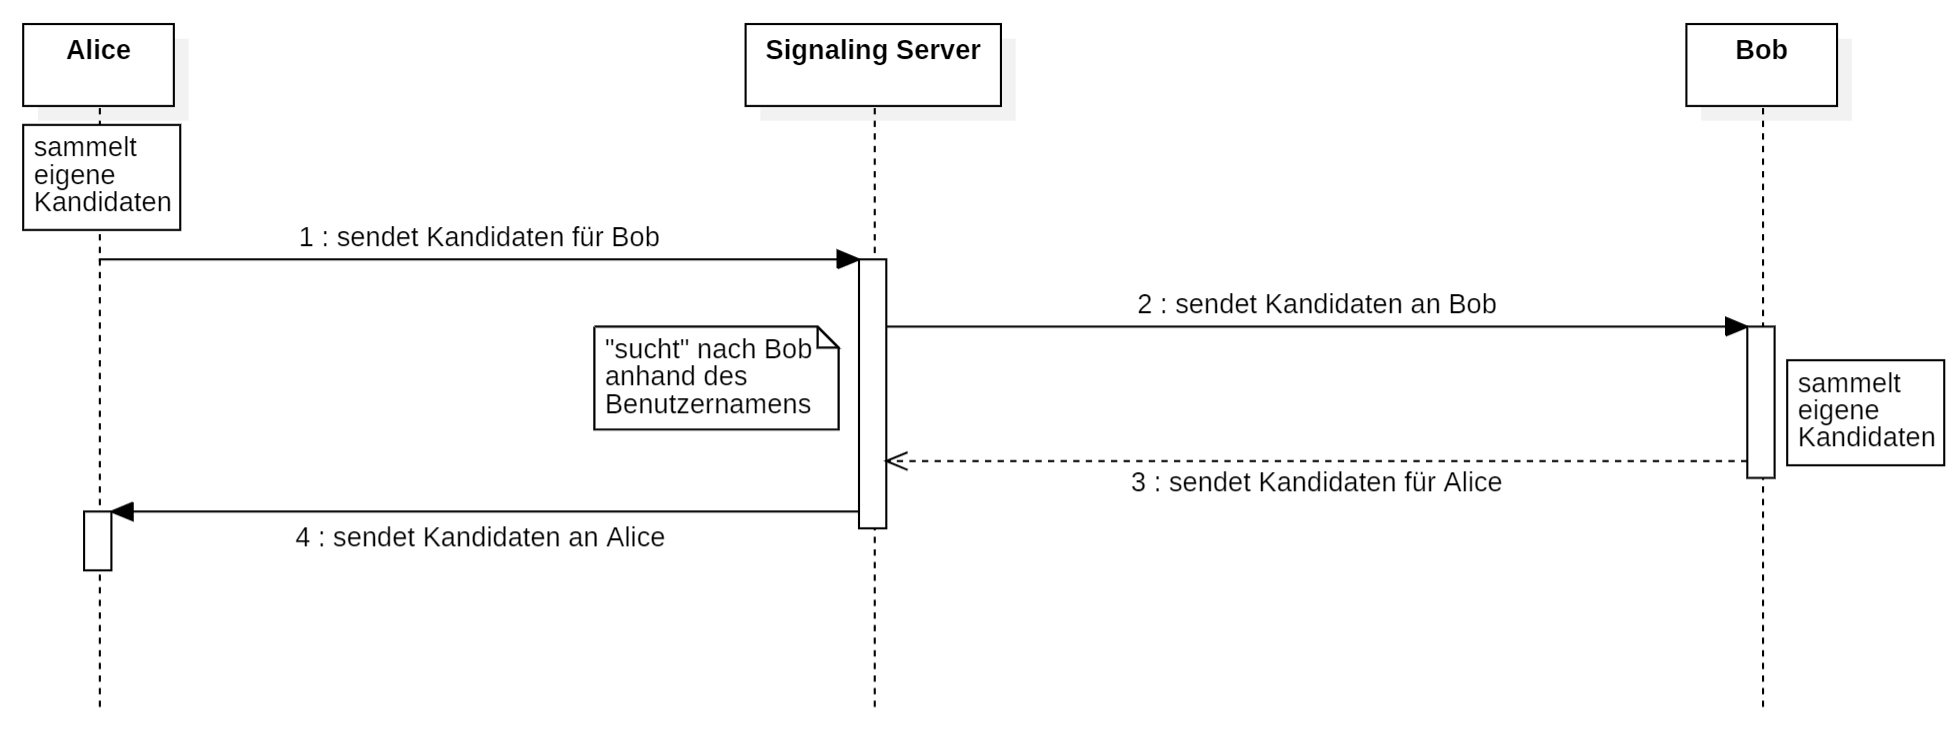
\includegraphics[width=1.0\linewidth]{images/signaling_sequence.png}
    \captionof{figure}{Kandidatenaustausch über einen Signaling Server}
    \label{fig:signaling_server}
\end{center}

\noindent Alice möchte eine Verbindung zu Bob aufbauen. Dazu sendet sie eine Verfügbarkeitsabfrage an den Signaling Server. Zusätzlich sendet sie ihre Kandidatenadressen mit, die sie zuvor gesammelt hat. Der Signaling Server erhält die Kandidatenadressen von Alice und prüft, ob Bob verfügbar ist. Wenn dies der Fall ist, sendet der Signaling Server die Kandidatenadressen von Alice an Bob. Bob speichert die Kandidatenadressen von Alice und sendet seine eigenen Kandidatenadressen an den Signaling Server. Der Signaling Server leitet diese dann an Alice weiter. Sollte Bob allerdings nicht verfügbar sein, sendet der Signaling Server eine Fehlermeldung an Alice. 

Man könnte nun argumentieren, dass Kademlia durch die Verwendung von ICE ersetzt wird, da auch ICE  die lokale IP-Adresse und den Port des Empfängers ermittelt und somit eine direkte Verbindung aufgebaut werden könnte. Doch Kademlia wird bewusst weiterhin verwendet, da es die Auslastung des Signaling Servers so gering wie möglich hält, indem der erste Versuch des Verbindungsaufbaus immer über Kademlia erfolgt. Erst wenn dieser fehlschlägt, wird das ICE-Protokoll verwendet, wodurch die Anzahl der Verbindungsversuche über den Signaling Server minimiert wird. Je nach Teilnehmeranzahl kann die Anzahl der Verbindungsversuche über den Signaling Server sehr hoch sein, was zu einer hohen Auslastung des Servers führen kann. Durch die Verwendung von Kademlia wird die Anzahl der Verbindungsversuche über den Signaling Server minimiert, da die Teilnehmer ihre Verbindungsadressen untereinander austauschen können, ohne den Signaling Server zu belasten.

In Phase zwei werden Konnektivitätsprüfungen durchgeführt. Diese Prüfungen dienen dazu, die Eignung und Zuverlässigkeit der gesammelten Verbindungswege zwischen den Geräten zu bewerten, um die bestmögliche Verbindung für eine erfolgreiche Kommunikation zu identifizieren. Die Reihenfolge der Konnektivitätsprüfungen wird durch einen Prioritätsalgorithmus bestimmt, der die Verbindungsadressen nach ihrer Priorität ordnet. Aus der Dokumentation von ICE geht hervor, dass die Priorität einer Verbindungsadresse durch die folgende Formel berechnet wird \parencite[S. 22]{rfc8445_ICE}:

\begin{equation}
    \label{eq:ice_priority}
    \text{priority} = \text{2}^{24} \cdot \text{(type preference)} + \text{2}^{8} \cdot \text{(local preference)} + \text{2}^{0} \cdot \text{(256 - component ID)}
\end{equation}

\noindent Jeder Kandidat hat eine Priorität, die durch die Formel \ref{eq:ice_priority} berechnet wird. Die Priorität wird durch die drei Werte in der Formel bestimmt: Typpräferenz, lokale Präferenz und Komponenten-ID. Die Typpräferenz ist ein Wert, der die Art der Verbindungsadresse angibt, und dessen Wert sich zwischen $0$ und $126$ befinden muss.
Es gibt, wie bereits in Phase eins aufgezeigt, drei verschiedene Typen von Verbindungsadressen: Host-Adressen, Peer-reflexive Adressen und Relay-Adressen.
Die Werte für die Typpräferenz, die in der Dokumentation von ICE für die Berechnung der Priorität empfohlen werden, sind die folgenden: $126$ für Host-Adressen, $100$ für Peer-reflexive Adressen und $0$ für Relay-Adressen. Wichtig ist, dass der Wert $0$ für Relay-Adressen nicht bedeutet, dass Relay-Adressen nicht verwendet werden sollten, sondern dass sie die niedrigste Priorität haben. Für das Protokoll dieser Arbeit werden diese Werte übernommen. Für die lokalen Präferenzen wird ein Wert von $65535$ empfohlen, um die Verwendung von lokalen Adressen zu priorisieren. Auch dieser Wert wird übernommen. Der dritte und letzte Wert der Formel ist die Komponenten-ID, die dazu dient, verschiedene Datenströme oder Komponenten innerhalb eines einzelnen Kandidaten zu unterscheiden. Das bedeutet, dass ein Kandidat mehrere Komponenten haben kann, die jeweils eine eigene Komponenten-ID haben. Dadurch können beispielweise Bild-Daten, Audio-Daten und Text-Daten innerhalb eines einzelnen Kandidaten über verschiedene Komponenten gesendet werden. Da in dem Protokoll dieser Arbeit nur ein Datenstrom verwendet wird - und zwar Text - wird der Komponenten-ID der Wert $1$ zugewiesen.

Wenn alle Kandidaten ihre Priorität erhalten haben, werden sie nach ihrer Priorität sortiert und die Konnektivitätsprüfung beginnt. Dieser Prozess beinhaltet den Versuch, Verbindungen aufzubauen und Datenverkehr über verschiedene potenzielle Wege zu senden und zu empfangen.
Durch das Senden von Probe-Paketen über jede potenzielle Verbindungsadresse wird geprüft, ob die Kommunikation erfolgreich erfolgen kann. Dabei werden die drei verschiedenen Arten von Adressen (lokale, reflexive und Relay-Adressen) verwendet, um verschiedene Möglichkeiten zu testen, wie die Geräte miteinander kommunizieren können. Die Probe-Pakete werden über UDP (User Datagram Protocol) gesendet, da es ein verbindungsloses Protokoll ist und somit vor dem Senden keine Verbindung aufgebaut werden muss \parencite[S. 1]{rfc768_UDP}. Dies ermöglicht es, die Erreichbarkeit der Verbindungsadressen zu testen, ohne eine Verbindung aufzubauen. Die Probe-Pakete werden an die Verbindungsadressen gesendet und die Antwort wird überwacht. Wenn eine Antwort empfangen wird, wird die Verbindungsadresse als erreichbar angesehen. Wenn keine Antwort empfangen wird, wird die Verbindungsadresse als nicht erreichbar angesehen. Die Probe-Pakete werden in regelmäßigen Abständen gesendet, um die Stabilität der Verbindungsadressen zu testen. Wenn die Probe-Pakete über einen längeren Zeitraum nicht beantwortet werden, wird die Verbindungsadresse als nicht stabil angesehen. 

Mit dem Abschluss der Konnektivitätsprüfungen beginnt die dritte und letzte Phase. Mit den Ergebnissen werden Kandidaten-Paare gebildet, die die Verbindungsadressen der beiden Geräte enthalten. Während dieses Schritts werden die gesammelten Kandidaten (lokale IP-Adressen, Ports und durch STUN oder TURN-Server erhaltene Reflexionen) in verschiedenen Konstellationen kombiniert. Jede dieser Kombinationen bildet ein Paar, das als möglicher Kommunikationsweg zwischen den Geräten dienen könnte. Die gebildeten Paare werden auf Redundanz kontrolliert und dann nach ihrer Priorität sortiert, die aus den einzelnen Prioritäten der Kandidaten berechnet wird. Aus dieser Reihenfolge wird dann die sogenannte \textit{Checkliste} erstellt, die die Paare in der Reihenfolge ihrer Priorität enthält. Auch die Kandidaten-Paare erhalten mit Hilfe einer Formel eine Priorität, die in der Dokumentation von ICE auf Seite 31 definiert ist \parencite[S. 31]{rfc8445_ICE}. Anschließend  wird damit begonnen, eine Verbindung über das Paar mit der höchsten Priorität aufzubauen. Wenn die Verbindung erfolgreich aufgebaut werden kann, wird die Kommunikation über dieses Paar fortgesetzt. Wenn die Verbindung nicht erfolgreich aufgebaut werden kann, wird das Paar mit der nächsthöheren Priorität ausgewählt und der Prozess wird wiederholt. Dieser Prozess wird fortgesetzt, bis eine Verbindung erfolgreich aufgebaut werden kann. Wenn keine Verbindung aufgebaut werden kann, wird die Kommunikation über das Paar mit der höchsten Priorität fortgesetzt, das eine Verbindung über den Relay-Server verwendet. Die folgenden Abbildung stellt den Ablauf des ICE-Prozesses bildlich, mit Hilfe eines Sequenzdiagramms, dar:

\begin{center}
    \captionsetup{type=figure}
    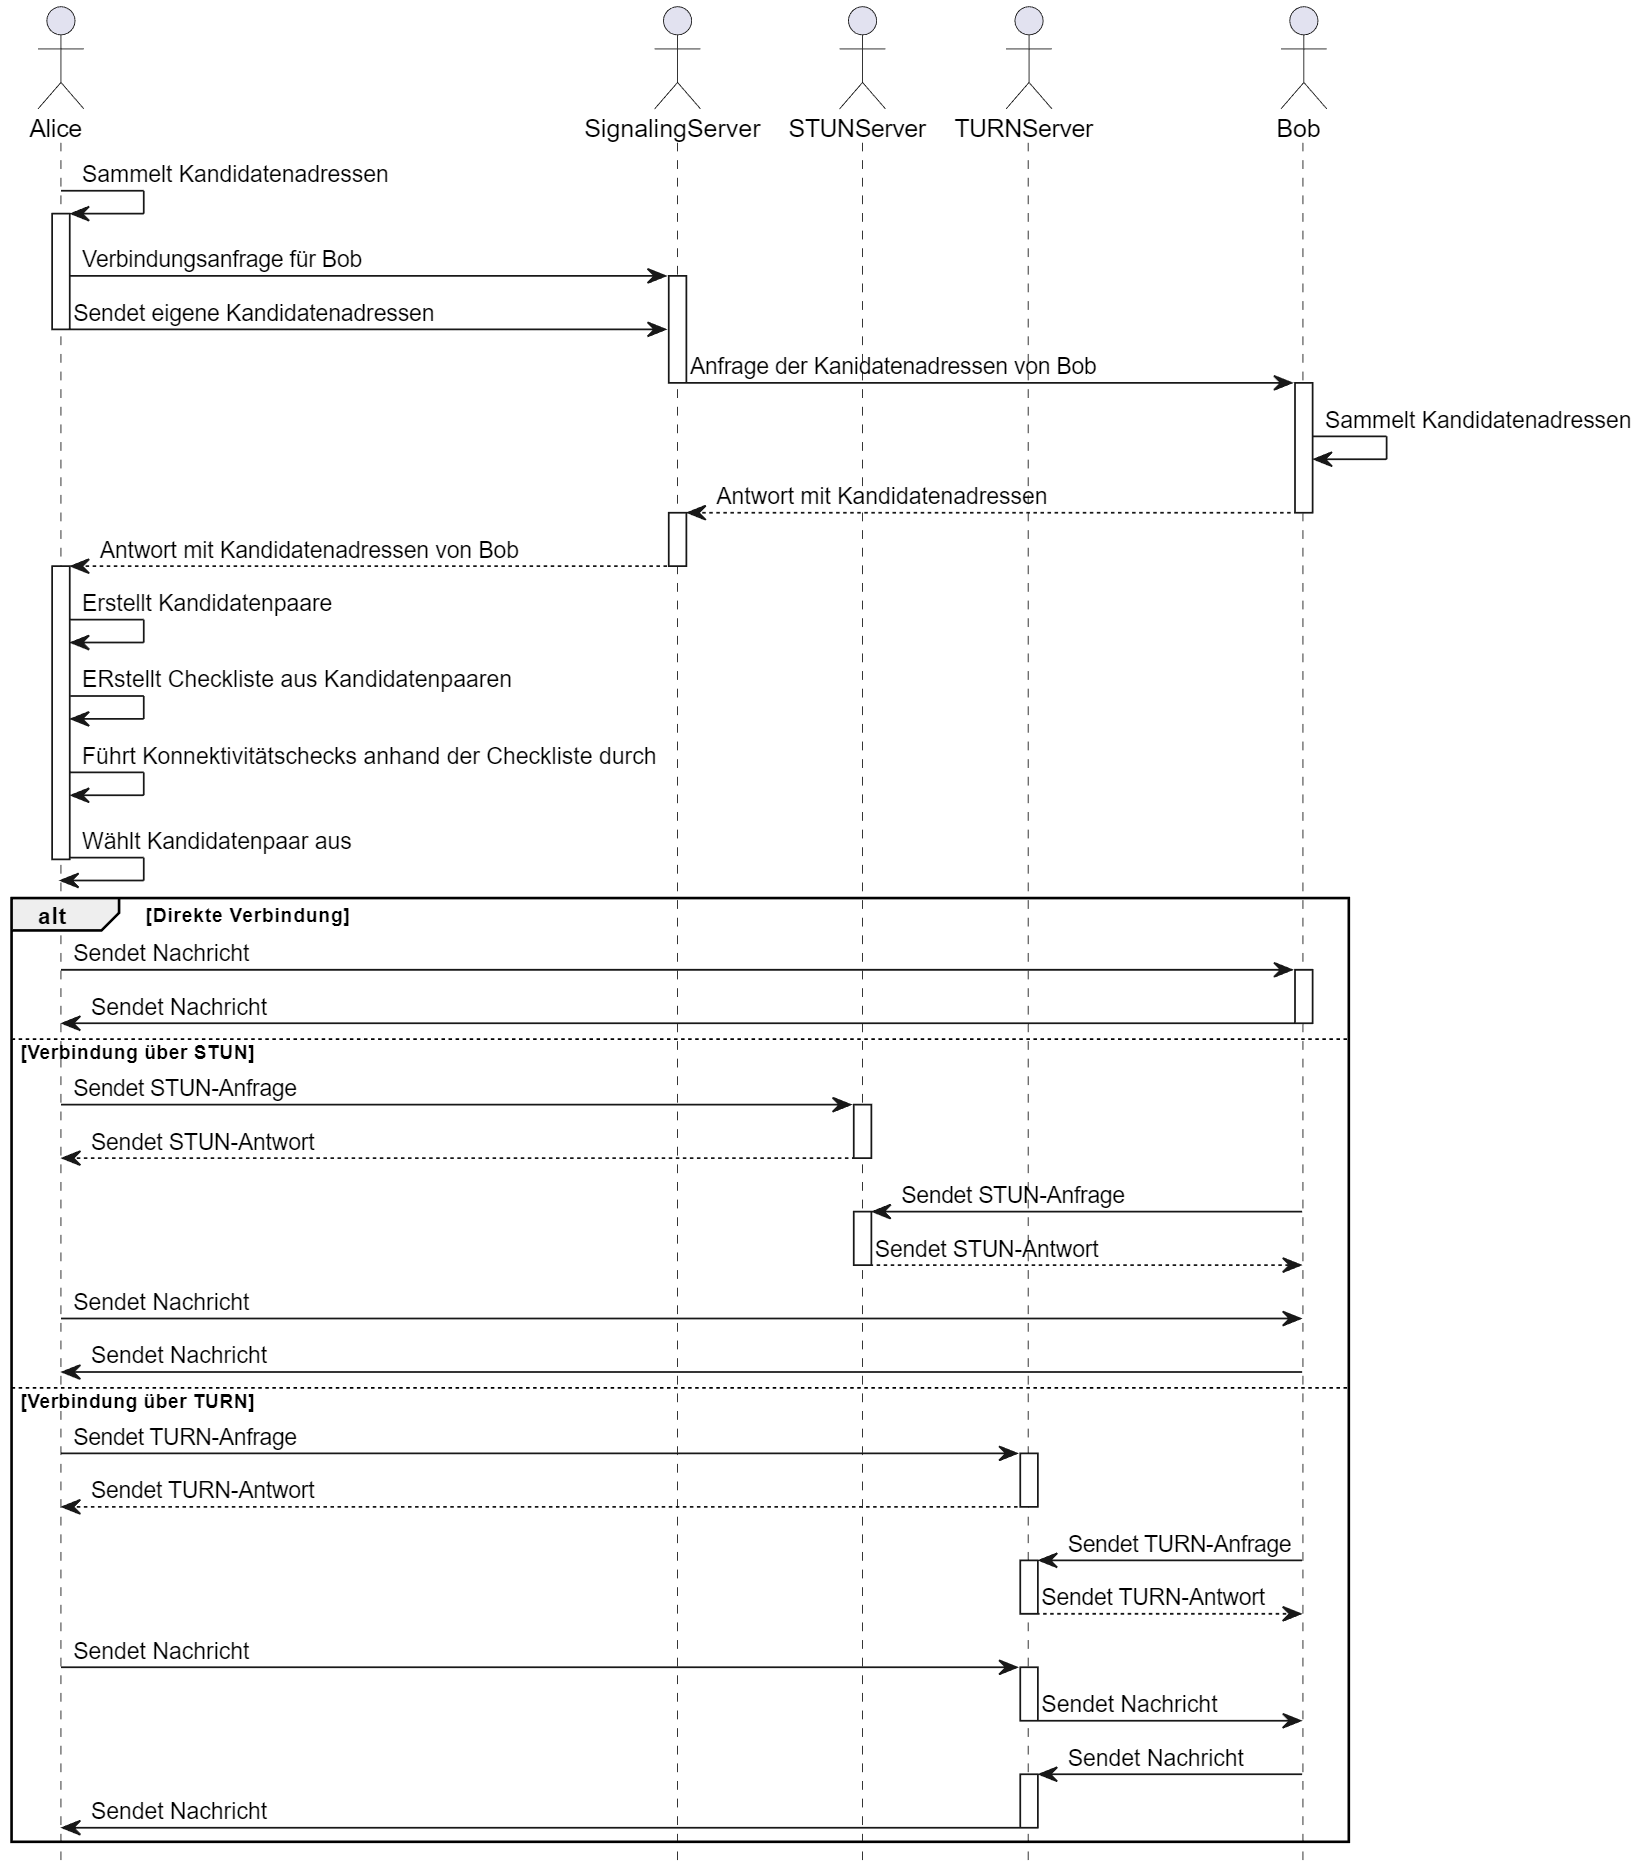
\includegraphics[width=1.0\linewidth]{images/ice_sequence.png}
    \captionof{figure}{ICE-Prozess}
    \label{fig:ice_sequence}
\end{center}

\noindent Ein großer Vorteil von ICE ist die Flexibilität, die es ermöglicht, sich an sich ändernde Netzwerkbedingungen anzupassen. Falls sich während der Kommunikation Netzwerkparameter ändern - beispielsweise durch einen Wechsel zwischen Wi-Fi und Mobilfunknetzwerken - kann ICE dynamisch neue Kandidatenadressen identifizieren und die Verbindungen anpassen, ohne die laufende Kommunikation zu unterbrechen.

\subsection{Nachrichtenübertragung}

Wenn die am besten geeignete Verbindungsadresse eine lokale Adresse ist, wird eine direkte Verbindung zwischen den Geräten aufgebaut. Wenn die am besten geeignete Verbindungsadresse eine reflexive Adresse ist, wird eine direkte Verbindung zwischen den Geräten aufgebaut, indem die reflexive Adresse als Zieladresse verwendet wird. Wenn wiederum die am besten geeignete Verbindungsadresse eine Relay-Adresse ist, wird eine Verbindung über den Relay-Server aufgebaut, indem die Relay-Adresse als Zieladresse verwendet wird. Der Nachrichtenaustausch erfolgt über die ausgewählte Verbindungsadresse. Wobei hier mit \textit{Verbindung aufbauen} gemeint ist, dass die Nachrichten über die Verbindungsadresse gesendet und empfangen werden können. Aus Sicht der Transportschicht wird durch die Verwendung von UDP keine Verbindung aufgebaut, denn UDP ist ein verbindungsloses Protokoll. Das bedeutet, dass keine Verbindung aufgebaut werden muss, um die Nachrichten zu senden und zu empfangen. Die Nachrichten werden über die Verbindungsadresse gesendet und empfangen. Aus Applikationssicht wird jedoch eine Verbindung aufgebaut, da die Nachrichten zwischen den Teilnehmern ausgetauscht werden können.
Ein Nachteil bei der Verwendung von UDP ist, dass die Nachrichten nicht zuverlässig zugestellt werden. Das bedeutet, dass Nachrichten verloren gehen können, ohne dass der Absender oder Empfänger davon erfährt. Das Transportprotokoll TCP (Transmission Control Protocol) hingegen ist zuverlässig, da es eine Verbindung aufbaut und sicherstellt, dass die Nachrichten erfolgreich zugestellt werden \parencite[S. 36]{rfc9293_TCP}. Im Falle von Paketverlusten ist auf der gleichen Seite definiert, dass TCP in der Lage ist, die verlorenen Pakete zu erkennen und erneut zu senden.

Doch eine mögliche Verwendung von TCP hat auch Nachteile: ein Nachteil ist, dass es eine Verbindung aufbauen muss, bevor die Nachrichten gesendet werden können. Dies kann zu einer höheren Latenz führen. Ein weiterer Nachteil ist, dass die Verbindung aufrechterhalten werden muss, um die Nachrichten zu senden und zu empfangen. Dies führt zu einem höheren Ressourcenverbrauch, da die Verbindung aufrechterhalten werden muss, auch wenn keine Nachrichten gesendet werden. Auch bei NATs hat TCP Nachteile. NATs schließen die Verbindungen nach einer gewissen Zeit, wenn keine Daten übertragen werden. Dies kann dazu führen, dass die Verbindung geschlossen werden, bevor die Nachrichten gesendet werden können. 
Ein überzeugendes Argument für die Verwendung von UDP liegt in seiner Effizienz durch den geringeren Overhead im Vergleich zu TCP. Dank des schlankeren Headers werden weniger Daten übertragen, was besonders in Instant Messaging-Szenarien, in denen kleine Nachrichten häufig versendet werden, zu einer effizienteren Nutzung der Netzwerkressourcen und zu schnelleren Übertragungen führt. UDP bietet zudem den Vorteil der Unabhängigkeit in Bezug auf die Reihenfolge der übermittelten Pakete. Im Gegensatz zu TCP, das die korrekte Reihenfolge sicherstellt, überlässt UDP diese Aufgabe der Anwendungsschicht. In Instant Messaging-Anwendungen, in denen die Reihenfolge der Nachrichten möglicherweise weniger kritisch ist, ermöglicht dies eine flexiblere und potenziell schnellere Übertragung von Nachrichten. Die geringere Verbindungsetablierungszeit von UDP ist ein weiterer Pluspunkt. Da UDP ein verbindungsloses Protokoll ist, entfällt der zeitliche Aufwand für das Auf- und Abbauen von Verbindungen. Dies ist besonders vorteilhaft in Umgebungen mit häufigen Verbindungswechseln, wie sie bei Instant-Messaging mittels Peer-to-Peer auftreten können. Die Minimierung der Latenzzeit trägt dazu bei, Nachrichten schneller bereitzustellen \parencites{rfc768_UDP}{rfc9293_TCP}. 
Aus diesen Gründen wurde UDP als Transportprotokoll für die Nachrichtenübertragung gewählt.


\subsection{Verbindungsabbau}

Da es wie bereits erwähnt keine Verbindung gibt, die aufgebaut werden muss, um die Nachrichten zu senden und zu empfangen, gibt es auch keinen Verbindungsabbau. Die Nachrichtenübertragung kann jederzeit gestoppt werden, indem einfach keine Nachrichten mehr gesendet werden. 

\section{Nachrichtenformat}
\label{sec:nachrichtenformat}


Jedes Instant-Messaging-Protokoll benötigt die Definition eines Nachrichtenformats, das die Struktur der Nachrichten festlegt, die zwischen den Teilnehmern ausgetauscht werden. Im Folgenden wird das Nachrichtenformat für das Instant-Messaging-Protokoll beschrieben.
Nachdem eine Verbindung zwischen zwei Teilnehmern hergestellt werden konnte, kann die Nachricht vom Sender an den Empfänger gesendet werden. Die Nachricht wird in binär serialisierter Form übertragen und enthält die folgenden Informationen:

\begin{itemize}
    \item Benutzername des Senders
    \item Benutzername des Empfängers
    \item Timestamp
    \item Signatur
    \item Nachrichtenlänge
    \item Nachrichteninhalt
\end{itemize}

\noindent Bei der Erstellung des Nachrichtenformats wurde sich an \cite[S. 9]{rfc2779_IMPP} orientiert. Die Benutzernamen erlauben die Zuordnung der Nachricht. Der Timestamp enthält die aktuelle Zeit, zu der die Nachricht gesendet wird und wird für die richtige Sortierung der Nachrichten verwendet. Die Signatur dient der Authentifizierung des Senders (siehe \ref{subsec:vertrauliche_kommunikation} \textit{\nameref{subsec:vertrauliche_kommunikation}}). Aus Sicherheitsgründen wird jede Nachricht signiert. Die Nachrichtenlänge gibt die Länge des Nachrichteninhalts an und der Nachrichteninhalt enthält die eigentliche Nachricht, die vom Sender an den Empfänger gesendet werden soll.


\section{Sicherheit}
\label{subsec:sicherheit}

% #TODO: Sessions könnten so ca. 10 Minuten dauern, dann wird ein neuer symmetrischer Schlüssel ausgehandelt
% Diffie-Hellman-Schlüsselaustausch basiert auf Gruppen, die aus einem Generator und einer Primzahl bestehen. Die Gruppen werden so gewählt, dass der diskrete Logarithmus in diesen Gruppen schwer zu berechnen ist. Der diskrete Logarithmus ist das inverse Element der Exponentialfunktion. Das bedeutet, dass der diskrete Logarithmus die Lösung der Gleichung $g^x = y$ ist, wobei $g$ der Generator, $x$ der diskrete Logarithmus und $y$ das Ergebnis der Exponentialfunktion ist. Die Schwierigkeit des diskreten Logarithmus ist, dass es keine effiziente Methode gibt, um ihn zu berechnen. Die Sicherheit des Diffie-Hellman-Schlüsselaustauschs basiert auf der Annahme, dass es keine effiziente Methode gibt, um den diskreten Logarithmus zu berechnen. Eine Gruppe kann aber auch aus einem elliptischen Kurvenpunkt und einer Primzahl bestehen. Die Sicherheit des Diffie-Hellman-Schlüsselaustauschs basiert auf der Annahme, dass es keine effiziente Methode gibt, um das diskrete Logarithmusproblem in elliptischen Kurven zu lösen.



\textcolor{red}{Quellenangaben, falls nicht schon in Grundlagen gemacht}


\noindent Um die Kommunikation zwischen den Teilnehmern zu schützen, wird sowohl asymmetrische als auch symmetrische Verschlüsselung verwendet. Die asymmetrische Verschlüsselung wird für die Authentifizierung und die symmetrische Verschlüsselung für die Ende-zu-Ende-Verschlüsselung der Nachrichten verwendet. Die asymmetrische Verschlüsselung wird mit Hilfe von Public-Key-Kryptographie realisiert. In dem von Whitfield Diffie und Martin Hellman 1976 veröffentlichten Paper \textit{New Directions in Cryptography} \parencite{DiffieHellman_NewDirectionsInCryptography} wurde die Public-Key-Kryptographie erstmals beschrieben. Darin wird die Problematik der symmetrischen Verschlüsselung beschrieben, dass ein Schlüssel für die Verschlüsselung und Entschlüsselung verwendet wird und dieser Schlüssel zu Beginn der Kommunikation über einen unsicheren Kanal  zwischen den Teilnehmern ausgetauscht werden muss. Die Lösung dieses Problems ist die Public-Key-Kryptographie.


Bei der Public-Key-Kryptographie wird ein Schlüsselpaar generiert, das aus einem öffentlichen und einem privaten Schlüssel besteht. In diesem Protokoll wird bei der Registrierung eines Teilnehmers ein statisches Schlüsselpaar generiert. Der öffentliche Schlüssel dieses Schlüsselpaars wird gemeinsam mit dem Benutzernamen in der Blockchain hinterlegt und der private Schlüssel wird lokal auf dem Gerät des Teilnehmers gespeichert.

Um die Ende-zu-Ende-Verschlüsselung zu realisieren, wird ein Diffie-Hellman Schlüsselaustausch durchgeführt, der auf elliptischen Kurven basiert und daher auch Elliptic-Curve-Diffie-Hellman-Schlüsselaustausch (oder kurz ECDH) genannt wird. Als Grundlage für einen Schlüsselaustausch muss sich auf eine gemeinsame elliptische Kurvengleichung geeinigt werden. Für das hier entwickelte Protokoll wird die Funktion \textit{X448} verwendet, die in RFC 7748 \textit{The X25519 and X448 Elliptic Curves} \parencite{rfc_ellipticCurves} spezifiziert ist.



Der Diffie-Hellman-Schlüsselaustausch basiert auf der Annahme, dass es keine effiziente Methode gibt, um den diskreten Logarithmus zu berechnen. Der Diffie-Hellman-Schlüsselaustausch basiert auf Gruppen, die aus einem Generator und einer Primzahl bestehen. Die Gruppen werden so gewählt, dass der diskrete Logarithmus in diesen Gruppen schwer zu berechnen ist. Der diskrete Logarithmus ist das inverse Element der Exponentialfunktion. Das bedeutet, dass der diskrete Logarithmus die Lösung der Gleichung $g^x = y$ ist, wobei $g$ der Generator, $x$ der diskrete Logarithmus und $y$ das Ergebnis der Exponentialfunktion ist. Die Schwierigkeit des diskreten Logarithmus ist, dass es keine effiziente Methode gibt, um ihn zu berechnen. Eine Gruppe kann aber auch aus einem elliptischen Kurvenpunkt und einer Primzahl bestehen. Die Sicherheit des Diffie-Hellman-Schlüsselaustauschs basiert auf der Annahme, dass es keine effiziente Methode gibt, um das diskrete Logarithmusproblem in elliptischen Kurven zu lösen.




Bei einem Verbindungsaufbau wird vom Sender ein neues Schlüsselpaar generiert, welches diesmal aus flüchtigen Schlüsseln besteht. Der Sender generiert einen flüchtigen privaten Schlüssel und einen flüchtigen öffentlichen Schlüssel. Der flüchtige öffentliche Schlüssel wird zusammen mit der ID des Senders und einem Zeitstempel in einer Nachricht, welche mit dem statischen privaten Schlüssel des Senders signiert wird, an den Empfänger gesendet. Der Empfänger kann die Nachricht mit dem öffentlichen Schlüssel des Senders, welcher mittels Smart Contract aus der Blockchain ausgelesen werden kann, entschlüsseln und somit die Authentizität des Senders verifizieren. Dadurch kann der Empfänger sicher sein, dass die Nachricht vom Sender stammt und nicht von einem Angreifer manipuliert wurde. Mit Hilfe des Zeitstempels kann der Empfänger außerdem feststellen, ob der flüchtige öffentliche Schlüssel noch gültig ist. Der Empfänger extrahiert den flüchtigen öffentlichen Schlüssel aus der Nachricht des Senders und ist somit im Besitz des flüchtigen öffentlichen Schlüssels des Senders. Der Empfänger generiert ebenfalls einen flüchtigen privaten Schlüssel und einen flüchtigen öffentlichen Schlüssel. Der flüchtige öffentliche Schlüssel wird zusammen mit der ID des Empfängers und einem Zeitstempel in einer Nachricht, welche mit dem statischen privaten Schlüssel des Empfängers signiert wird, an den Sender gesendet. Der Sender kann die Nachricht mit dem öffentlichen Schlüssel des Empfängers entschlüsseln und somit die Authentizität des Empfängers verifizieren. Nun sind beide Teilnehmer im Besitz des flüchtigen öffentlichen Schlüssels des jeweils anderen Teilnehmers.


Anschließend wird ein gemeinsamer geheimer Schlüssel aus dem flüchtigen privaten Schlüssel und dem öffentlichen Schlüssel des Empfängers mittels Key-Derivation-Funktion berechnet und die flüchtigen Schlüssel werden verworfen. Der berechnete flüchtige symmetrische Schlüssel wird für die Verschlüsselung der Nachrichten verwendet.

Durch die Anwendung von flüchtigen Schlüsseln wird die Sicherheit erhöht, da diese nur für eine kurze Zeit existieren und somit ein Angreifer nur für einen kurzen Zeitraum Zugriff auf diese hat. Mit Hilfe dieser Methode wird eine Ende-zu-Ende-Verschlüsselung ermöglicht, da nur der Sender und der Empfänger den gemeinsamen geheimen Schlüssel kennen. Selbst wenn die Verbindung über ein Relay läuft, kann dieses die Nachricht nicht entschlüsseln, da es den gemeinsamen geheimen Schlüssel nicht kennt. Die Verwendung von flüchtigen Schlüsseln hat jedoch auch Nachteile. So muss bei jedem Verbindungsaufbau ein neues Schlüsselpaar generiert werden, was einen erhöhten Rechenaufwand bedeutet. 



\section{Integration von Blockchain}
\label{sec:blockchainintegration}


\subsection{Auswahl der Blockchain}
Für die Integration der Blockchain in das Protokoll wurde zunächst eine geeignete Blockchain gesucht. Dabei wurde sich auf die beiden bekanntesten Blockchains, Bitcoin und Ethereum, beschränkt. Da Bitcoin eine reine Kryptowährung ist und keine Smart Contracts unterstützt, wurde sich für Ethereum entschieden. Ethereum ist eine Blockchain, die zwar auch eine Kryptowährung, Ether, besitzt, aber zusätzlich auch Smart Contracts unterstützt. Der Grund für die Existenz einer Währung auf der Blockchain ist, dass die Smart Contracts, die auf der Blockchain ausgeführt werden, mit Ether bezahlt werden müssen \parencite[S. 2]{Antonopoulos_MasteringEthereum}. Somit ist es nicht möglich, Smart Contracts auf der Blockchain auszuführen, ohne Ether zu besitzen. Da die Smart Contracts auf der Blockchain aber mit Ether bezahlt werden müssen, ist es notwendig, dass jeder Nutzer, der einen Smart Contract ausführen möchte, Ether besitzt.


\subsection{Registrierung}
Um das Protokoll zu nutzen, muss sich jeder Nutzer zunächst auf der Blockchain registrieren. Dazu muss ein Smart Contract auf der Blockchain ausgeführt werden, der die Registrierung des Nutzers durchführt. Dieser Smart Contract wird mit dem Benutzernamen und dem statischen öffentlichen Schlüssel aufgerufen. Der statische öffentliche Schlüssel wird bei der Registrierung festgelegt und kann nicht mehr geändert werden. Der Smart Contract erstellt einen neuen Eintrag in der Blockchain, der den Benutzernamen und den öffentlichen Schlüssel des Nutzers enthält. Der Smart Contract wird nur einmalig bei der Registrierung aufgerufen. Sollte ein Nutzer seinen Benutzernamen ändern wollen, muss er sich mit dem neuen Benutzernamen und dem öffentlichen Schlüssel eines neu erzeugten statischen Schlüsselpaars erneut registrieren.
% Der alte Benutzername wird dann aus der Blockchain gelöscht. -> wie könnte man das absichern?

\subsection{Kommunikation}
Für die Kommunikation mit anderen Teilnehmern, muss zunächst die ID des anderen Teilnehmers im Kademlia-Netzwerk bekannt sein. Dazu wird der Benutzername des anderen Teilnehmers auf der Blockchain gesucht um zu kontrollieren, ob dieser bereits registriert ist. Ist der Benutzername nicht auf der Blockchain vorhanden, ist der andere Teilnehmer nicht registriert und es kann keine Verbindung aufgebaut werden. Ist der Benutzername auf der Blockchain vorhanden, wird der dazugehörige öffentliche Schlüssel ausgelesen. Der Benutzername entspricht gleichzeitig der ID des Teilnehmers im Kademlia-Netzwerk. Somit kann der Verbindungsaufbau, der in Abschnitt \ref{subsec:verbindungsmanagement} \nameref{subsec:verbindungsmanagement} beschrieben wird, durchgeführt werden.
Wenn der Verbindungsaufbau erfolgreich war, kann die Kommunikation beginnen. Dazu wird der öffentliche Schlüssel des anderen Teilnehmers benötigt. Dieser wird ebenfalls auf der Blockchain gespeichert. Somit kann jeder Teilnehmer die öffentlichen Schlüssel der anderen Teilnehmer auf der Blockchain finden und die Nachrichten, die er erhält, mit dem öffentlichen Schlüssel des Absenders verifizieren. Somit kann sichergestellt werden, dass die Nachrichten tatsächlich vom angegebenen Absender stammen und nicht von einem anderen Teilnehmer gesendet wurden, der sich als jemand anderes ausgibt.

\subsection{Entwurf der Smart Contracts}
\label{subsec:smartcontracts}

Auf der Ethereum-Blockchain wird die hauptsächlich Programmiersprache Solidity verwendet, um Smart Contracts zu erstellen. Solidity ist eine objektorientierte Programmiersprache, die stark an JavaScript angelehnt ist \parencite[S. 131]{Antonopoulos_MasteringEthereum}. Die Smart Contracts, die für das Protokoll benötigt werden, sind in Solidity implementiert.


